\documentclass[dvipsnames,svgnames,x11names,margin=3pt]{standalone}
\usepackage{tikz,pgfplots,xparse,pgfmath,pgffor}
\pgfplotsset{compat = 1.18,width=10cm,height=10cm}

\begin{document}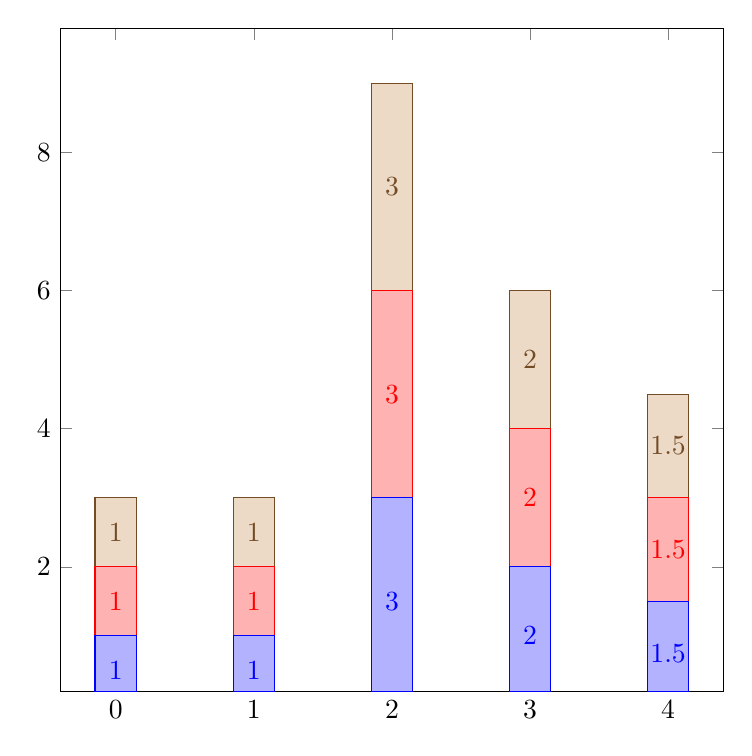
\begin{tikzpicture}

% stack plots=x：将图形堆叠在x方向上。即将具有相同x坐标的数据堆叠在一起。
% stack plots=y：将图形堆叠在y方向上。即将具有相同y坐标的数据堆叠在一起。
% stack plots=false：不进行堆叠，图形不会重叠在一起。
% xbar stacked=plus：将水平条形图进行堆叠，并以正值为基准。
% xbar stacked=minus：将水平条形图进行堆叠，并以负值为基准。
% stack dir=plus：在堆叠图形中，正值向上堆叠。
% stack dir=minus：在堆叠图形中，负值向上堆叠。
% reverse stacked plots=true：反转堆叠图形的堆叠顺序。
% reverse stacked plots=false：保持堆叠图形的默认堆叠顺序。
% stacked ignores zero=true：堆叠图形时忽略零值。
% stacked ignores zero=false：在堆叠图形时不忽略零值。
% xbar interval stacked=plus：将水平条形间隔图进行堆叠，并以正值为基准。
% xbar interval stacked=minus：将水平条形间隔图进行堆叠，并以负值为基准。
% bar width=0.4：设置条形图的宽度。
% nodes near coords：在图形上显示数据点的标签。
% stack negative=on previous：在堆叠图形中，负值按照前一个数据点进行堆叠。
% bar shift auto：自动调整条形图的位置，以避免重叠。

\begin{axis}[
    stack plots = y,
    /tikz/ybar,
    ybar stacked,
    bar width = 15pt,
    nodes near coords ]
\addplot coordinates {(0,1) (1,1) (2,3) (3,2) (4,1.5)};
\addplot coordinates {(0,1) (1,1) (2,3) (3,2) (4,1.5)};
\addplot coordinates {(0,1) (1,1) (2,3) (3,2) (4,1.5)};
\end{axis}

\end{tikzpicture}\end{document}